\setcounter{page}{67}
\begin{minipage}[10cm]{\textwidth}
    \setlength\columnsep{20pt}
    \setlength\parindent{24pt}
    \begin{multicols*}{2}
    10 к л а с с
    
    \begin{enumerate}[itemindent=32pt]
      \setlength{\itemsep}{0pt}
      \setlength{\parskip}{0pt}
      \setcounter{enumi}{4}
      
      \item См. задачу № 5 для 8-го класса.
      \item Докажите, что для любого тетраэдара существуют такие две плоскости, что отношение площадей проекций тетраэдра на эти плоскости не меньше $ \sqrt{2} $.
      \item Рассмотрим $n$ чисел $a_1, a_2, \dots, a_n$.
      Положим
    \[b_k = \frac{a_i + \dots + a_k}{k}  (\textrm{для } k = 1, 2, \dots) ,\] 
    \[C = (a_1 - b_1)^2 + (a_2 - b_2)^2  + \dots + (a_n - b_n)^2,\] 
    \[D = (a_1 - b_n)^2 + (a_2 - b_n)^2  + \dots + (a_n - b_n)^2. \]
    
    Докажите неравенства $ C \le D \le 2C $.
    
    \item Рассмотрим последовательность чисел $ x_n = (1 + \sqrt{2} + \sqrt{3})^n $.  Каждое из них приводится к виду
    \[ x_n = q_n + r_n\sqrt{2} + s_n\sqrt{3} + t_n\sqrt{6},\]
    где $q_n, r_n, s_n, t_n$ --- целые числа. Найдите пределы
    \[ \lim_{n\to\infty} \frac{r_n}{q_n},\quad \lim_{n\to\infty} \frac{s_n}{q_n}, \quad \lim_{n\to\infty} \frac{t_n}{q_n}. \]
    
    \item См. задачу № 8 для 9-го класса.
    \end{enumerate}
    
    Как участники соревнования справились с этими задачами, видно из приведенной таблицы. К сожалению, некоторые задачи оказались довольно трудными. Так, у восьмиклассников с задачей № 2 справились
\\
\null\hfill Т а б л и ц а 
\\
        \begin{tabular}{c|l|}
            \hline
            \rotatebox{90}{Результаты} & \multicolumn{1}{c}{Номера задач} \\
            \hline
             \rotatebox{270}{$+$ \rotatebox{90}{$\pm$} \rotatebox{90}{$\mp$}} &
                \begin{tabular}{cccccccccccc}
                     \multicolumn{12}{c}{\textbf{8 класс}} \\
                     1&2&3&4a&4б&5а&5б&5в&6&7а&7б&8 \\
                     \hline
                     15&2&1&26&2&24&17&4&7&4&2&4 \\
                     8&0&0&5&9&0&3&12&0&1&1&1 \\
                     2&0&0&0&5&0&2&4&1&1&2&2 \\
                \end{tabular} \\
             \rotatebox{270}{$+$ \rotatebox{90}{$\pm$} \rotatebox{90}{$\mp$}} & \begin{tabular}{ccccccccc}
                     \multicolumn{9}{c}{\textbf{9 класс}} \\
                     1&2&3а&3б&4&5&6&7&8 \\
                     \hline
                     44&9&17&2&0&23&23&9&6 \\
                     13&0&2&2&0&14&1&1&0 \\
                     0&1&1&3&5&11&1&4&1 \\
                \end{tabular} \\
            \rotatebox{270}{$+$ \rotatebox{90}{$\pm$} \rotatebox{90}{$\mp$}} & \begin{tabular}{ccccccccccc}
                     \multicolumn{11}{c}{\textbf{10 класс}} \\
                     1&2&3а&3б&3в&4&5&6&7&8&9 \\
                     \hline
                     42&12&29&11&1&1&23&5&6&11&2\\
                     2&4&2&3&2&0&11&1&2&7&0 \\
                     0&2&4&9&1&17&2&5&4&9&0 \\
                \end{tabular} \\
        \end{tabular}
\\
\\
только два школьника, с задачей № 3 --- один школьник и с задачей № 8 --- четыре школьника. 
    
Никто из девятиклассников не решил задачи № 4 и только два человека полностью решили задачу № 3б.
    
Среди десятиклассников задачи № 3в и 4 полностью решили толь-
    \end{multicols*}
\end{minipage}

\begin{SCfigure}[][h]
\caption{\textbf{Восьмиклассники, награжденные Дипломами 1 степени (слева направо): Ю. Ткаченко, А. Балинский, А. Разборов, А. Боричев.}}
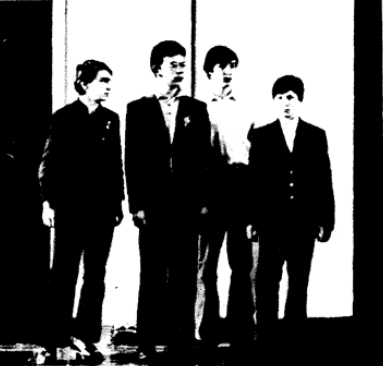
\includegraphics[scale=1]{winners.png}
\end{SCfigure}